\section{Introduction}
\subsection{Problem Background}
Energy is the significant material basis of economic growth and social development. As the major energy production and consumption power in the world, the U.S. state government attaches great importance to energy policy. The establishment of a interstate new energy contract not only helps to strengthen the cooperation between the states and jointly promote the sustainable, multivariate  and clean development of energy but also satisfies the energy demand of the economic development of various industries.

California (CA), Arizona (AZ), New Mexico (NM) and Texas (Texas) plan to create a new realistic energy compact. We are tasked with conducting data analysis to model on the basis of what is known in all four states, and setting a series of goals for new energy contract which focused on cleaner and renewable energy.

Faced with the following difficulties, we try to find some solutions:
\begin{enumerate}[\bfseries 1.]
	\item	Analyze the overall situation of energy in four states according to the data in the table.
	\item	Develop a model to describe the energy profiles and analyze the similarities and differences of the four states.
	\item	Establish standards to evaluate the use of cleaner and renewable energy.
	\item	Build a forecasting model and Making predictions about the future energy situation.
	\item	set goals for interstate energy contract based on the results of the four questions above.
	\item	Identify effective actions to achieve the goal.
	\item	Summarize a memo to Governors.
\end{enumerate}

\subsection{Analysis and Approach Overview}
Any serious statistical analysis begins with substantial work on the data. The data provided had a panoply of issues ranging from energy price, energy production,energy consumption to GDP, factor, and price.

For problem 1, due to the hugeness of data, we only select several important and representative data for analysis. We mainly choose the energy consumption.

For problem 2, in order to take both the overall and individual characteristics into account which is precisely the feature of longitudinal data analysis, we develop the energy profile model based on hierarchical linear. Then by solving and analyzing the result, we can get the similarities and differences in four states. The reason is analyzed in combination with the actual situation, such as geography, industry, population, and climate.

For problem 3, to fully assess the use of cleaner and renewable energy of four states, we combine the three variables in the table, eliminate the influence of dimensionality through normalization and then calculate the weighted sum of these three indexes as assessment criteria.  To solve forecasting problem 4, we consider regression models and make

linear fitting for historical data of all kinds of energy.

For problem 5.6.7, the solutions are based on the results of the first four questions.

\section{Assumptions}
In order to simplify the course of modeling and draw some reasonable conclusions from our model, we make assumptions as follows
\begin{enumerate}
\item	We assume that the data given by the title is true and reliable, the impact of human factors on the data is not considered.
\item 	We assume that the data given by the title is true and reliable, the impact of human factors on the data is not considered.
\end{enumerate}

\section{Symbols and Notations}
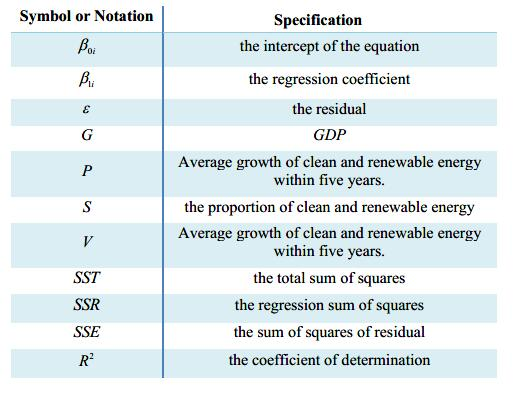
\includegraphics[width=0.6\paperwidth]{images/notation.jpg}

\section{Energy profile of four states}
There are a lot of variables in the dataset. And we select nine representative indicators to analyze the energy profile of four states.We list them as follows:

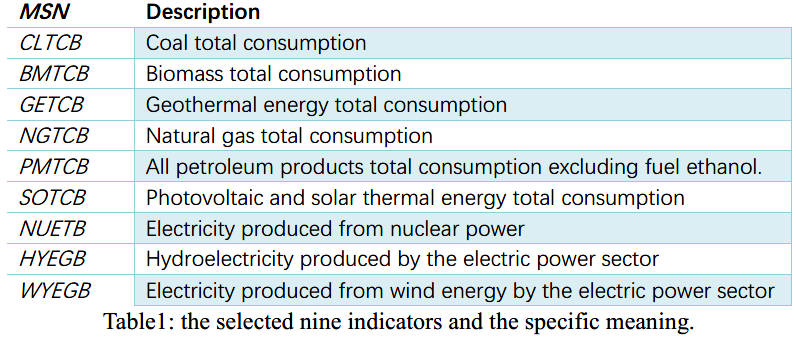
\includegraphics[width=0.6\paperwidth]{images/table1.png}

From the data, we can easily see that energy consumption in the four continents shows a slight fluctuation and a slow rise in 1960-2009.

Depicted below are graphs of the evolution of Arizona��s energy consumption structure.
\begin{figure}[b]
	\centering
	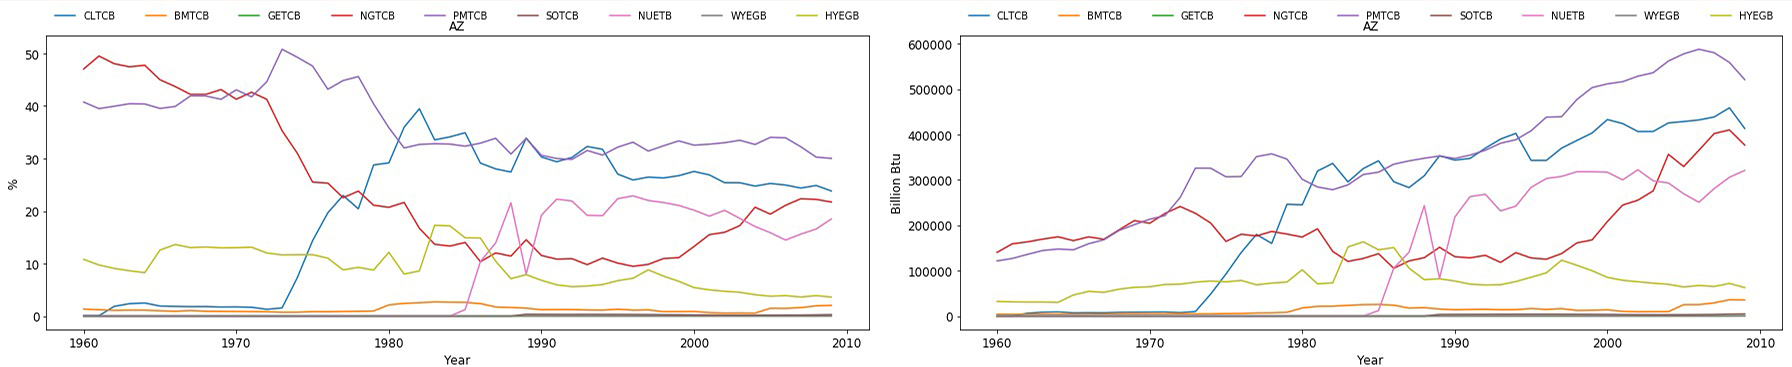
\includegraphics[width=0.7\paperwidth]{images/figure1.jpg}
	\caption{The change of the proportion of energy consumption, (left) vs. the change of the value of energy consumption (right) in Arizona, and the abscissa is the year.}
\end{figure}

As can be seen from table 1, the overall trend in Arizona (AZ) shows that the usage of all kinds of energy is on the rise.  During the 1960s and the 1970s, oil and natural gas were the main components, and the proportion of both of them accounted for more than 95\% of the total energy consumption. After the 1970s�� oil crisis, the usage of coal was constantly improving. Then the proportion reached 43.19\% in the whole energy structure in 1982. By 1985 nuclear power begins to be adopted. However, the momentum of nuclear power plant�� development was blocked because of Three Mile Island and Chernobyl accident in 1986, but then quickly restored to the original state. After 2000, the four main energy consumption was basically stable.

The chart below shows a variation of the California energy consumption structure.
\begin{figure}[h]
	\centering
	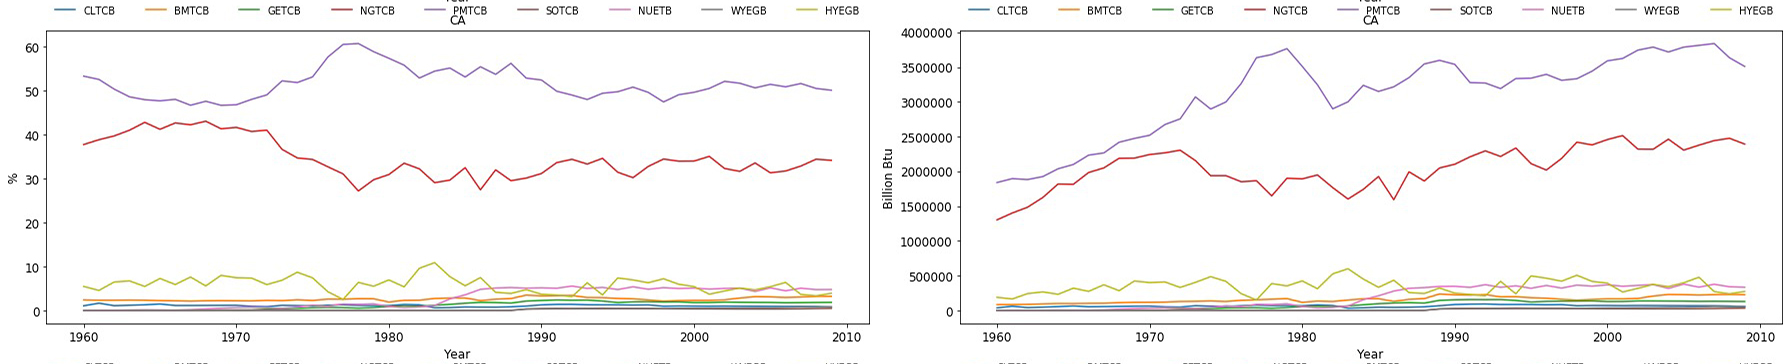
\includegraphics[width=0.7\paperwidth]{images/figure2.jpg}
	\caption{The change of the proportion of energy consumption, (left) vs. the change of the value of energy consumption (right) in California, and the abscissa is the year.}
\end{figure}

As we can see from Figure 2, the two fossil fuels, oil and gas, are the main sources of energy in California (CA). In 1960 the proportion of oil and natural gas in the energy consumption structure has already up to 56.42\% and 39.94\%. Even in 2009 they were still 52.62\% and 35.86\% , far more than other sources of energy and took the absolute advantage. Over the past 50 years their use has been increasing year by year. .At the same time, it can be seen that in the mid-1980s, the usage of nuclear energy increased slowly, and remained around 5\% in the later period. In addition, other types of energy consumption are very small.

New Mexico energy consumption structure changes as below:
\begin{figure}[h]
	\centering
	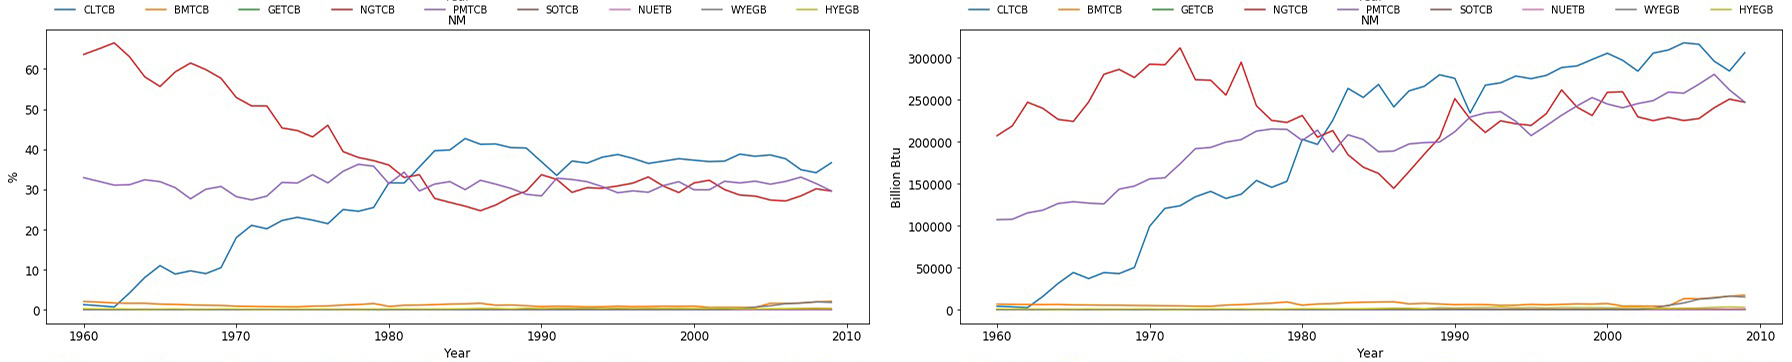
\includegraphics[width=0.7\paperwidth]{images/figure3.jpg}
	\caption{The change of the proportion of energy consumption, (left) vs. the change of the value of energy consumption (right) in New Mexico, and the abscissa is the year.}
\end{figure}

It can be seen from figure 3 that at first New Mexico (NM) mainly used gas and oil. The proportion of coal increased in the energy consumption structure, which has risen from 1.25\% in 1960 to 37.40\% in 2009. Ultimately, the three are relatively stable in the overall energy ratio. The consumption of oil and coal increases over time, while natural gas fluctuates in a large range, and overall consumption does not change much. Other sources of energy account for very little of the whole energy.

The chart below shows the change of Texas energy structure.

\begin{figure}[h]
	\centering
	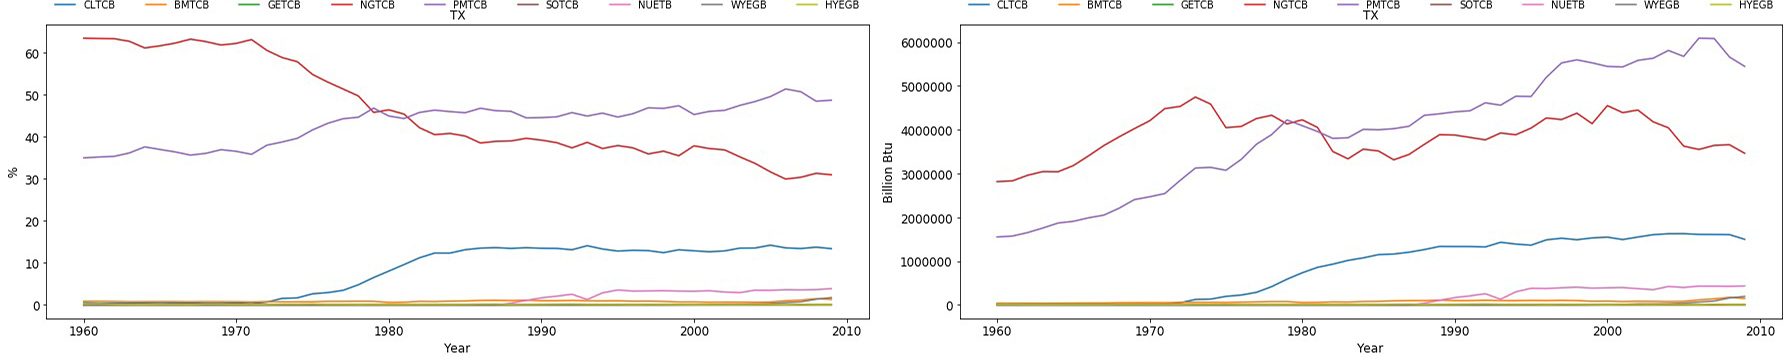
\includegraphics[width=0.7\paperwidth]{images/figure4.jpg}
	\caption{The change of the proportion of energy consumption, (left) vs. the change of the value of energy consumption (right) in Texas, and the abscissa is the year.}
\end{figure}

Texas initially used two kinds of fossil fuels, natural gas and oil, and their proportion in the whole energy consumption structure was 63.54\% and 35.03\% respectively in 1960.

In the middle of 70s, the usage of coal began to increase, and the proportion in the whole energy consumption structure also increased gradually. It reached 13.53\% in 1986, and after that remained stable. The consumption of oil is increasing year by year, eventually replacing natural gas and becoming the most used energy in Dirk Seth. Nuclear energy began to be used in the late 90s, but the scale is small, and the proportion is only about 4\%.

\section{Energy Profile Model}
Our task is to build a model that describes the energy profiles of four states from 1960 to 2009.

The data provided in the dataset is a longitudinal data, which is a repeated measure of the four states that can reflect the energy profile. In the analysis of longitudinal data, we mainly focus on two problems, one is to describe the overall average growth trend, and the other is to describe the differences in the growth trend among different individuals.

For the characteristics of longitudinal data., we adopt the energy profile model based on hierarchical linear. The hierarchical linear model can not only analyze the overall average growth trend, but also pay attention to the differences between individual development trend and explain the reasons for the difference. That is to say, our model can describe the four states�� development general situation of the energy, from 1960 to 2009, and also provide some parameters to illustrate the similarities and differences between states.

\subsection{The establishment of a double-layer model}
In order to better reflect the energy profile of the four states, as well as the use of cleaner and renewable energy, we develop a double - layer linear model. The first layer shows the overall situation of energy, and the second layer can express the consumption and change trend of cleaner and renewable energy. Here is a brief introduction to the principles of the double-layer linear model.

To start with, in the first layer of data structure, taking tracking observation results as dependent variables and observing time as independent variables, we establish the first layer regression equation:

\begin{equation}
\label{e1}
Y_{ij} = \beta_{0i} + \beta_{1i}X_{ij} + \varepsilon_{ij}
\end{equation}

In the equation, the subscript $0, 1, i$ and $j$ means the intercept, the slope, the sequence number of the observed object and the number of times of observation.$\beta_{0i}$  is the intercept of the equation, whose meaning is the average of this observation. $\beta_{1i}$  is the regression coefficient, which represents the rate of change of the observation. $X$ represents the value of the independent variables. $\varepsilon$  is on behalf of the residual, meaning the part that the measured value $Y$ cannot be explained by the independent variable $X$.

In the second layer, we build two second-floor regression equations with the intercept and slope of the equation (\ref{e1})  as the independent variable, the individual characteristics of the observed objects or the experiments accepted as dependent variables. It is as follows:

\begin{align}
\beta_{0i} = \gamma_{00} + \gamma_{01}W_{1i} + \mu_{0i} \label{e2} \\
\beta_{1i} = \gamma_{10} + \gamma_{11}W_{li} + \mu_{1i} \label{e3}
\end{align}

Some of the variables in the equation can be listed as below:

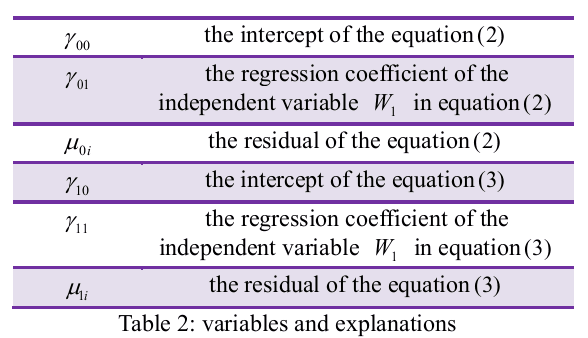
\includegraphics[width=0.6\paperwidth]{images/table2.png}

\subsection{The solution of model}
Taking California for example, we use the nine variables��s corresponding energy consumption and proportion every five years to create two data files (  by SPSS statistic software). The contents of the two files are as follows.

\begin{figure}[h]
	\centering
	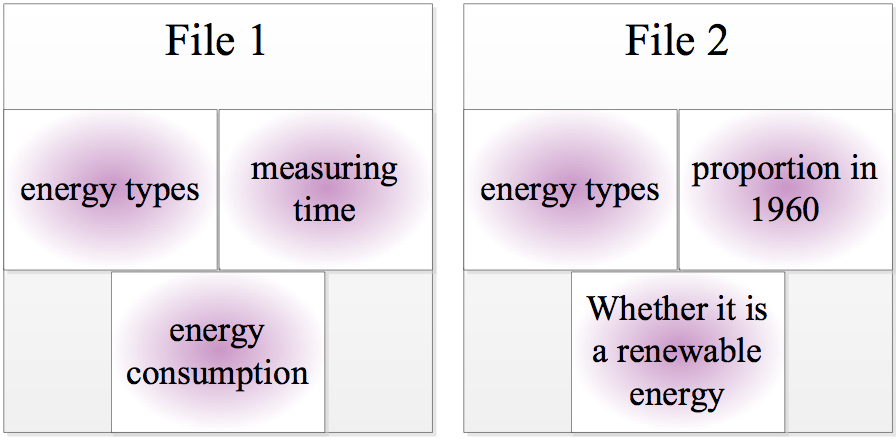
\includegraphics{images/figure5.png}
	\caption{the contents of the two files}
\end{figure}

In the double-layer model, the equation of the first layer is.
\begin{equation}
Y = \beta_0 + \beta_1 \times t + \varepsilon
\end{equation}

the equation of the second layer is

\begin{align}
\beta_{0} = \gamma_{00} + A\gamma_{01} + B\gamma_{02} + \mu_0 \\
\beta_{1} = \gamma_{10} + A\gamma_{11} + B\gamma_{12} + \mu_1
\end{align}

The specific meanings of each variable in the energy profile model are listed below:

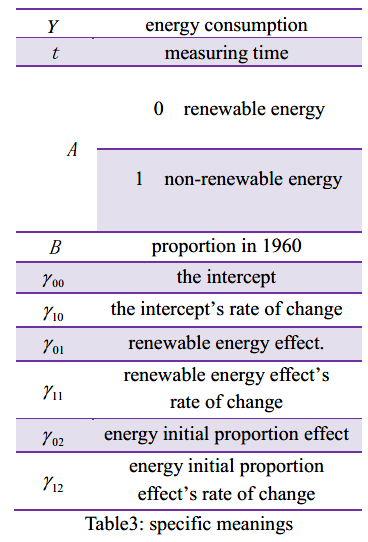
\includegraphics[width=0.5\paperwidth]{images/table3.png}

In addition, considering the energy proportion'score is 0 to 10, in order to explain conveniently, we centralized energy proportion. After parameter estimation(by HLM6.0), the results are shown in table4:

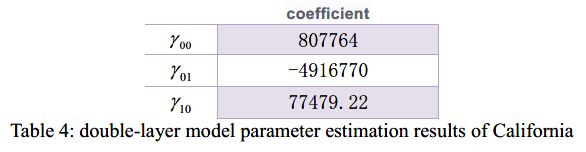
\includegraphics[width=0.6\paperwidth]{images/table4.png}

The chart has shown that the current energy consumption of clean energy is 807764 billion btu, which is 491,6770 billion btu lower than non-clean energy and the energy consumption trend of clean energy is increased by 77479 billion btu every five years, with an average growth rate of 16.02\%.

Data from the remaining three states were shown in table 5:

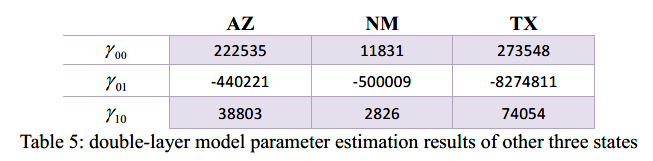
\includegraphics[width=0.6\paperwidth]{images/table5.png}

From the above table, we can know that the four states of energy is similar in the constant improvement of clean energy consumption and the possession of proportion in the whole energy structure also increases year by year. While the development speed is relatively slow, for the reason that the high cost of the use of renewable energy and people still tend to use fossil fuels.The entire energy structure is still dominated by non-renewable energy sources such as oil, gas and coal, which is expected to continue for some time.

The differences between the four states are that there are more people in California and Texas, so they consume more energy than the other two states.They develop different types of clean energy, such as California, which has plenty of light and is suitable for the development of solar energy. Arizona is rich in water resources and can promote hydropower generation.Texas has rich wind energy, which can boost its use of wind power. And New Mexico is rich in most energy, so the development of cleaner and renewable energy is slow compared to other states.

\section{Performance evaluation model for cleaner, renewable energy}
To determine which of the four states�� performance of using cleaner, renewable energy in 2009 is the best, we build an index to quantify their use of clean and renewable sources of energy, which is convenient for our choice.

On the basis of existing data in the dataset,  we can easily find that there are three indicators well reflecting the four states��s use condition of cleaner and renewable energy in 2009. They are GDP, the ratio of cleaner and renewable energy to total energy consumption and the average growth of cleaner and renewable energy in the last five years of each state. And the weighted sum of these three indexes is what we want.

\subsection{Reasons for choice}
By referring to relevant information,we find that growth of GDP leads to increase in energy demand and consumptive endogeneity. Thus, the value of GDP reflects the energy consumption. Through cleaner and renewable energy use accounting for the proportion of total energy consumption��s statistics, we can compare it visually. The average growth can help us learn about the potential for clean and renewable energy in the future.

\subsection{The establishment of indicators}
In the following equation, the variables and their meanings are as bellow:

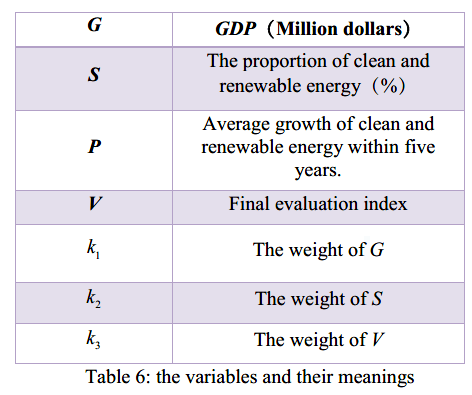
\includegraphics[width=0.6\paperwidth]{images/table6.png}

\begin{equation}
V = k_1G + k_2S + k_3P
\end{equation}

The results of three indicators are calculated as follows:

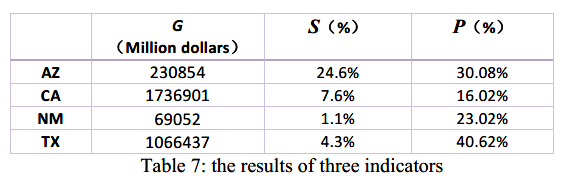
\includegraphics[width=0.6\paperwidth]{images/table7.png}

In order to eliminate the influence of dimension and data value range on the result, we normalized the data:

\begin{equation}
x^* = \dfrac{x-min}{max-min}
\end{equation}

We take $k_1=0.1, k_2 =0.7, k_3 =0.2$ ,calculating the states' $V$ as below:

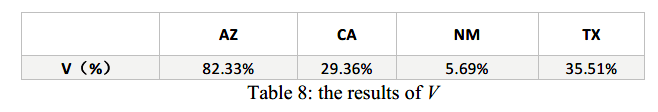
\includegraphics[width=0.6\paperwidth]{images/table8.png}

The results show that Arizona used clean energy and renewable energy in 2009, showing the best effect.

\section{Linear regression prediction analysis}
In order to make predictions about the energy profile of four states in 2025 and 2050 without any policy changes, we make linear fitting for historical data of all kinds of energy.

Regression analysis is a statistical analysis method to determine the quantitative relationship between two or more variables. If there is only one independent variable and one dependent variable included, and the relationship between the two can be approximated by a straight line, then we call it linear regression analysisy.

Now we define the symbol. We define X as the independent variable in which case X is the year and Y as the dependent variable, namely the value of the energy type that needs to be predicted. a and b is the correlation coefficient. Linear regression expressions are as follows:

$$Y = aX+b$$

To obtain a, b, we need to solve  $\min Q(a, b)$:

$$\min Q(a, b) = \sum_{i=1}^n(Y_i - (aX_i+b))^2$$

Reduce it to get: 
$$Q(a, b) = n\overline{Y^2} - 2an\overline{XY} - 2bn\overline Y + a^2n\overline{X^2} + 2abn\overline X + nb^2$$

To get the minimum of $Q(a, b)$ , we find the partial derivatives of $Q$ for $a$ and $Q$ for $b$ , then make it all zero.

$$ \frac{\partial Q}{\partial a} = -2n\overline{XY} + 2an\overline{X^2} + 2bn\overline X = 0 $$
$$ \frac{\partial Q}{\partial b} = -2n\overline Y  + 2an\overline X + 2nb = 0 $$

Then we get the formula:
$$ a = \dfrac{\overline X \overline Y - \overline{XY}}{(\overline X)^2 - \overline{X^2}} $$
$$ b = \overline Y - a\overline X $$

We use the  (the coefficient of determination) to determine the fitting degree of the regression equation.

The total sum of squares (proportional to the variance of the data):
$$SST = \sum_{i=1}^n(Y_i - \overline Y)^2$$

The regression sum of squares, also called the explained sum of squares
$$SSR = \sum_{i=1}^n (\hat {Y_i} - \overline Y)^2$$

The sum of squares of residuals, also called the residual sum of squares:
$$SSE = \sum_{i=1}^n (\hat {Y_i} - Y_i)^2 = \sum_{i=1}^n e_i^2$$

The most general definition of the coefficient of determination is
$$R^2 = 1 - \frac{SSE}{SST}$$

The partial fitting curve are as follows.
\begin{figure}[b]
	\centering
	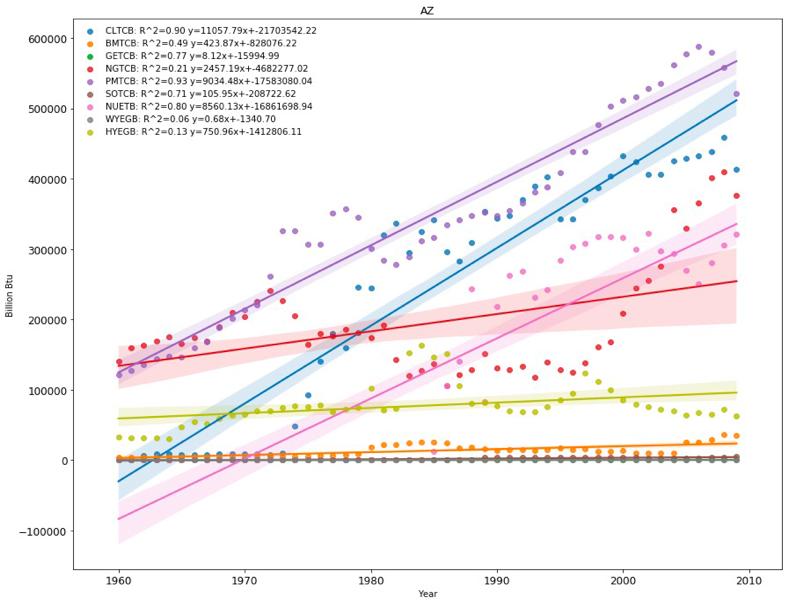
\includegraphics{images/figure6.png}
	\caption{Fitting curve of Arizona}
\end{figure}

\begin{figure}[h]
	\centering
	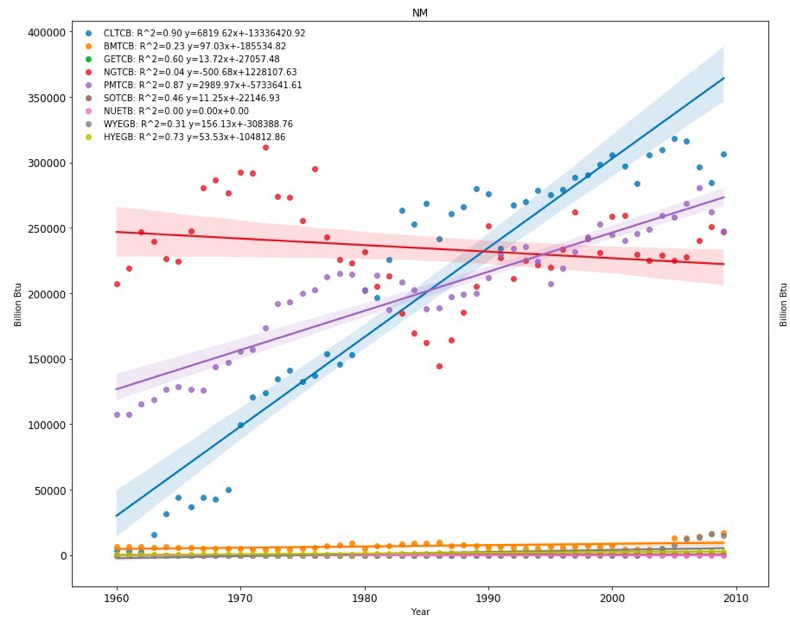
\includegraphics{images/figure7.png}
	\caption{Fitting curve of New Mexico}
\end{figure}

Finally, we have the following results and we listed the partial of them:

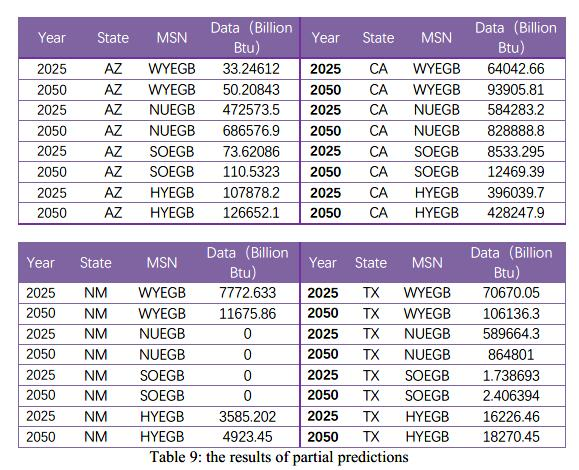
\includegraphics[width=0.6\paperwidth]{images/table9.jpg}

\section{The goals for renewable energy use in 2025 and 2050}
In the first part, we have predicted the energy profile of eachstate in 2025 and 2050, as well as the proportion of renewable energy in the whole energy structure system. The results can be listed as bellow:

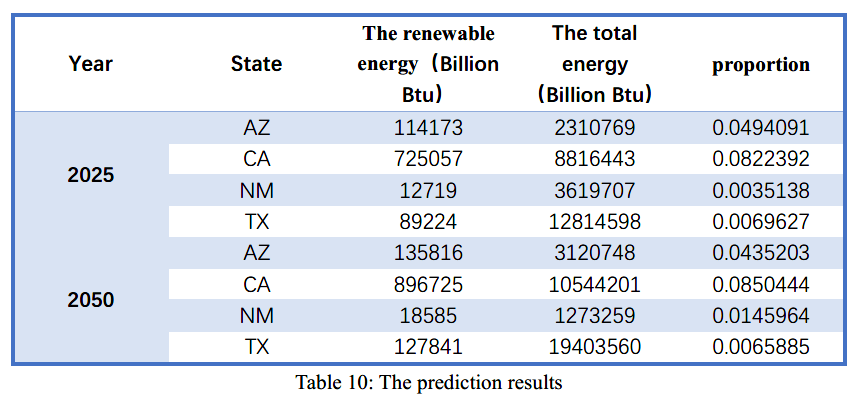
\includegraphics[width=0.6\paperwidth]{images/table10.png}

As can be seen from the above table 10, the predicted value of renewable energy is very small in the whole energy structure, which may be due to the small base of renewable energy and the insufficient growth of renewable energy in the initial stage. But for the development of the future energy structure, this circumstance is not science.According to the best standard, referring to a five-year average growth, the proportion of renewable energy in the whole energy of four areas in 2025 and 2025 are as shown in table 11:

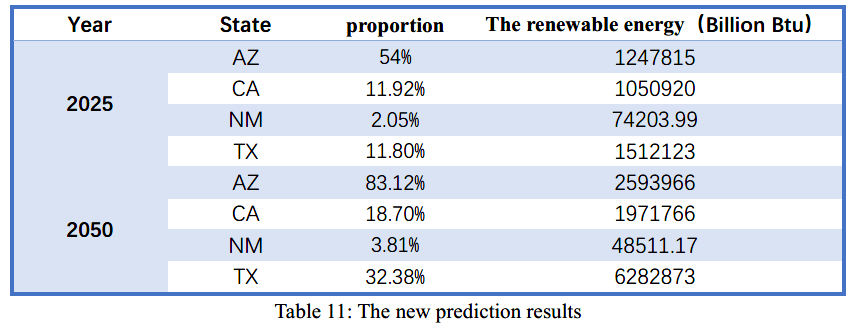
\includegraphics[width=0.6\paperwidth]{images/table11.png}

The new renewable energy sources will be added to the renewable energy targets in 2025 and 2050, and the goals we got are 3885061 billion btu and 10897115 billion btu.

\section{Three actions}
\begin{enumerate}
	\item Increase the number of large-scale production equipment, which can aggrandize the capacity of renewable energy in a relatively short time.
	\item Sign the purchase agreement of electricity for large orders and obtain renewable energy sources elsewhere.
	\item Develop a diversified energy collection model and make full use of renewable energy resources.
\end{enumerate}

\section{The Conclusion}
In our study, we have done lots of data processing work, putting forward the energy profile model. We also constructed a cleaner, renewable energy evaluation index which can be used to quantify the states�� use of clean and renewable sources of energy.In addition, we made predictions about the energy profile and set goals for the interstate energy agreement.

\section{Summary memorandum}
 Introduce the  total energy consumption,   the proportion of clean energy  proportion in the whole energy structure and its growth rate from 1960 to 2009, let the audience can have a general knowledge of energy situation.

 What is the development trend of different types of energy?  Seize the tide of The Times.

 With the absence of any policy changes, my forecast of the use of renewable energy will reach 941173 Billion Btu and 118967 Billion Btu in 2025 and 2050.

 We suggest that the new energy target be set in a higher level, which will be 3885061 Billion Btu and 10897115 Billion Btu in 2025 and 2050.


\begin{thebibliography}{99}
\addcontentsline{toc}{section}{References}  %���ò��ֱ��⣨"Refenrence"����������
\bibitem{1}	zhang xu. Analysis of multi-energy system model based on regional energy supply [D]. Shanghai jiaotong university,2015
\bibitem{2}	zhang long. Research on performance evaluation of renewable energy development [D]. China university of geosciences,2017
\bibitem{3} \texttt{https://www.jianshu.com/p/fcd220697182}
\end{thebibliography}

